\documentclass[12pt]{article}

\usepackage[T2A]{fontenc}
\usepackage[utf8]{inputenc}
\usepackage[russian]{babel}

\usepackage{mathtext}
\usepackage{cmap}
\usepackage{amsmath,amssymb,amsthm,amscd,amsfonts}
\usepackage{graphicx}
\usepackage[colorbox,usenames,dvipsnames]{xcolor}
\usepackage{float, caption, subcaption, multirow}
\usepackage[section]{minted}
\usepackage{hyperref}
\usepackage{multirow}

\voffset -24.5mm
\hoffset -5mm
\textwidth 173mm
\textheight 240mm
\oddsidemargin=0mm \evensidemargin=0mm

\definecolor{codegray}{gray}{0.9}
\newcommand{\code}[1]{\colorbox{codegray}{\texttt{#1}}}
\newmintinline[src]{java}{}

\renewcommand{\theFancyVerbLine}{\sffamily\textcolor{black}{\scriptsize\oldstylenums{\arabic{FancyVerbLine}}}}
\usemintedstyle[java]{tango}
\setminted[java] {
     bgcolor = codegray,
     linenos = true,
     tabsize = 2,
     formatcom = \color{black},
     frame = leftline,
     framerule = 0.8pt,
     framesep = 0.5cm,
     xleftmargin = 1cm,
     breaklines = true,
     escapeinside=||
}

\begin{document}

\title{Отчет по дисциплине \\ <<Параллельные вычисления>>} 
\author{Евгений Хандыго, гр. 53501/3}

\maketitle
\tableofcontents

\newpage

\section{Постановка задачи}

В рамках данной работы необходимо решить задачу вычисления площади фигуры, состоящей из произвольного набора окружностей
(возможно пересекающихся) методом \emph{Монте-Карло} (\emph{Monte-Carclo}). Решение задачи должно быть представлено в виде программы на 
языке \texttt{C++} или \texttt{Java}. При этом реализация программы должна предусматривать использование соедующих подходов:
\begin{itemize}
    \item Последовательный.
    \item Параллельный, с использованием стандартных средств управления потоками выбранного языка программирования.
    \item Параллельный, с использованием парадигмы \texttt{OpenMP} или \texttt{MPI}.
\end{itemize}

Результаты работы необходимо представить в виде статистики замеров времени исполнения различных решений и их сравнения. Также 
необходимо провести комплексное тестирование разработанных програм для доказания корректности их работы.
\section{Введение}

Метод Монте-Карло в общем случае применяется для приближенного вычисления интегралов (фактически) произвольной сложности. Суть метода
заключается в том, чтобы оценить плотность распределения, график которой в точности равен подинтегральной функции. Таким образом, 
метод Монте-Карло в некотором роде коррелирует с методом \emph{выборки с отклонением} (\emph{rejective sampling}). 

Мы здесь не будем вдаваться в детали данного метода, опишем лишь алгоритм оценки меры произвольной фигуры методом Монте-Карло:
\begin{enumerate}
    \item Фигура, меру которой необходимо оценить, заключается в другую фигуру, которая:
        \begin{itemize}
            \item <<Достаточно>> оптимальна с точки зрения минимальности замыкающей фигуры.
            \item Может быть <<легко>> использована в качестве области определения для генератора равномерно распределнных точек.
        \end{itemize}  
    \item В замыкающей фигуре генерирутеся <<достаточно>> большое число $n$ равномерно распределенных точек. Для каждой из точки 
        определяется попала ли она в фигуру, площадь которой необходимо вычислить.
    \item Производится подсчет количества точек ($m$), которые попали в фигуру, площадь которой необходимо вычислить. Тогда
        искомая величина может быть оценена по следующей формуле:
        \begin{equation*}
            S * \frac{m}{n},
        \end{equation*}
        где $S$ --- площадь замыкающей фигуры.
\end{enumerate}
В дополнение к описанному алгоритму заметим, что точность метода Монте-Карло является величиной порядка $\frac{1}{n^2}$, что в свою 
очередь делает $n$ <<достаточно>> хорошим при значениях порядка $10^3$. Понятно, что в общем случае (например, если оцениваемая фигура 
сильно разряжена) может потребоваться и гораздо большее количество экспериментов.
\section{Детали реализации}

В рамках данной работы было принято решения реализовать требуемые программы на языке \texttt{Java}. Для реализации третьего варианта 
решения задачи было решено использовать парадигму \texttt{MPI}, поскольку существует его расширения для языка программирования 
\texttt{Java} --- \texttt{MPJ Express Project} \footnote{http://mpj-express.org/index.html}. Данная реализация использует нативную
реализацию \texttt{MPI} через \texttt{Java Native Interface} (\texttt{JNI}).

Разработанный в рамках данной работы проект может быть разделен на следующие части:
\begin{itemize}
    \item Классы, описывающие геометрические фигуры и взаимоотношения меджу ними.
    \item Классы, реализующие непосредственно задачу оценки фигуры методом Монте-Карло.
    \item Классы, предназначенные для запуска экспериментов и сбора статистики.
    \item Тестовые классы.
\end{itemize}

Ниже на рисунках \ref{fig:geometry-class-diagram} -- \ref{fig:geometry-performance-diagram} представлены диаграммы классов основных 
частей проекта. 
\begin{figure}[H]
    \centering
    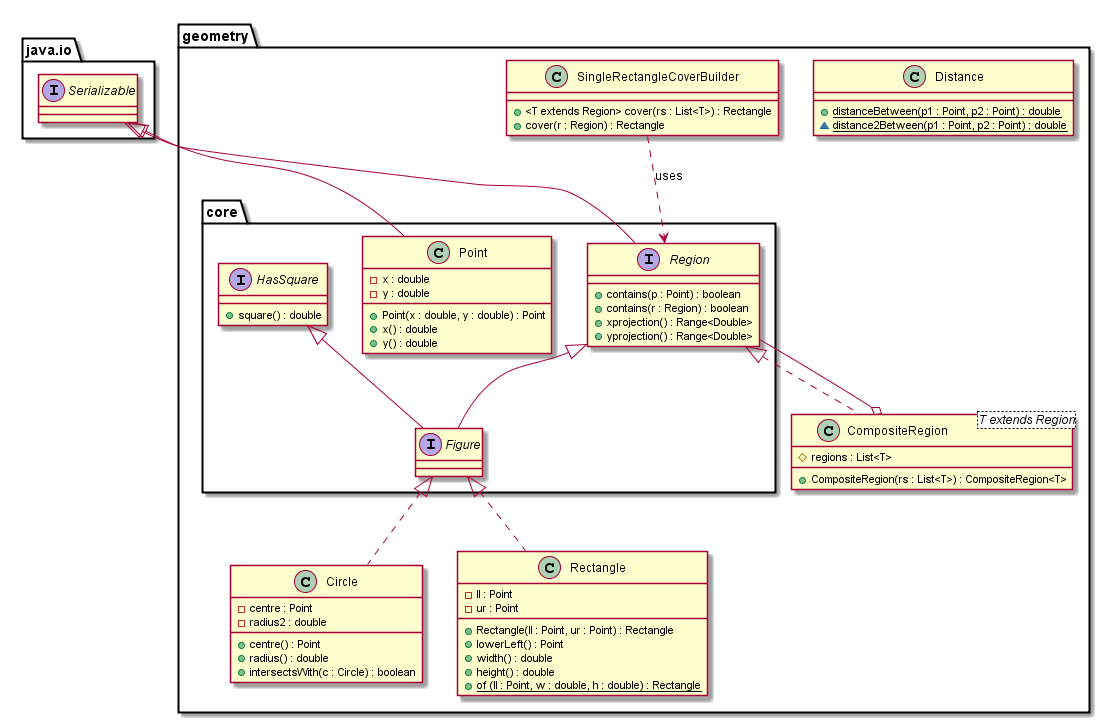
\includegraphics[width=18cm]{resources/diagrams/01_geometry.png}
    \caption{Диаграмма класов для пакета geometry}
    \label{fig:geometry-class-diagram}
\end{figure}
\\ \hfill \\ \hfill
\begin{figure}[H]
    \centering
    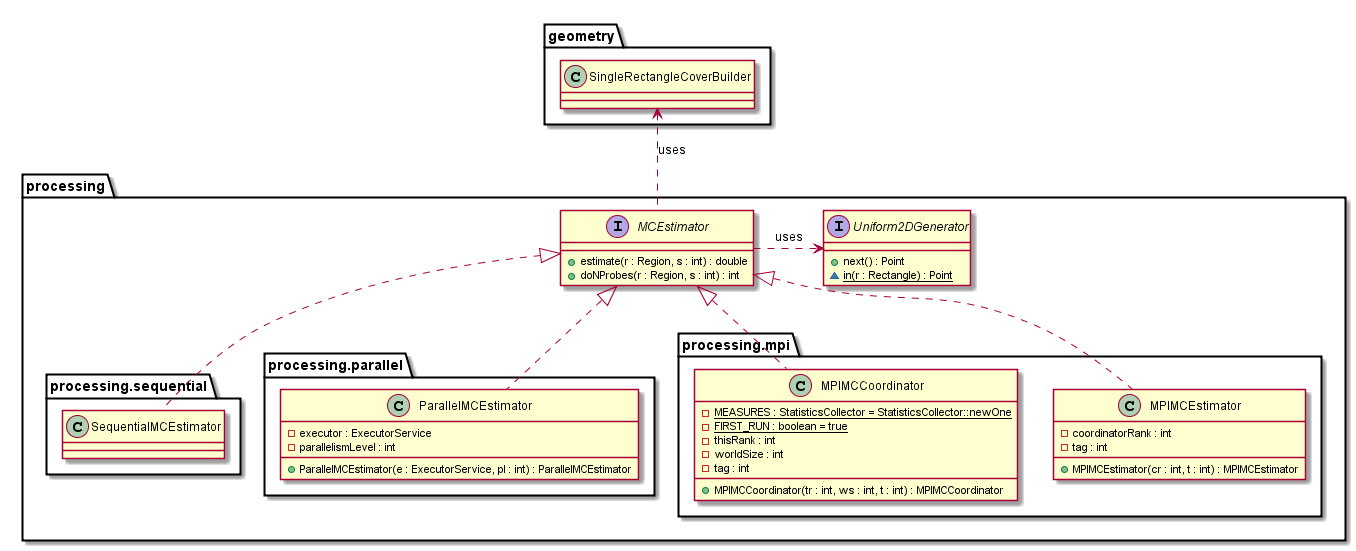
\includegraphics[width=23cm, angle=90]{resources/diagrams/02_processing.png}
    \caption{Диаграмма класов для пакета processing}
    \label{fig:geometry-processing-diagram}
\end{figure}

\begin{figure}[H]
    \centering
    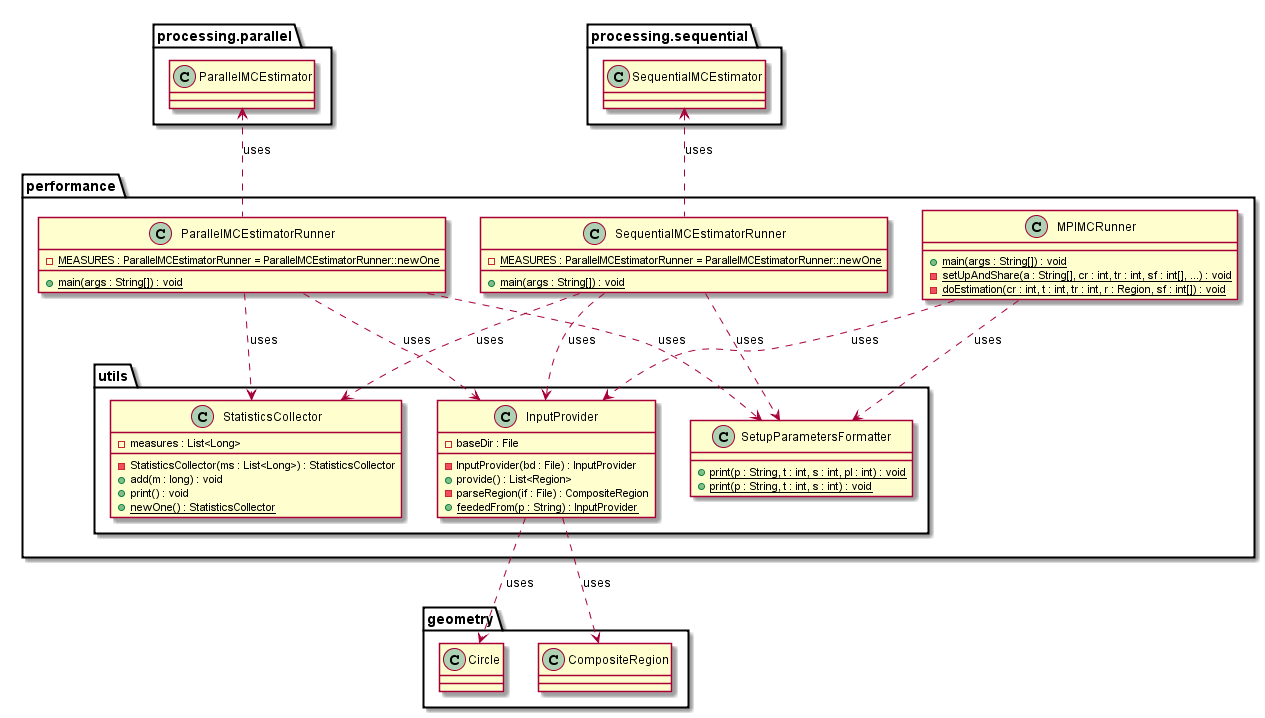
\includegraphics[width=23cm, angle=90]{resources/diagrams/03_performance.png}
    \caption{Диаграмма класов для пакета performance}
    \label{fig:geometry-performance-diagram}
\end{figure}

Ниже в листинге \ref{lst:mc-estimator-src} приведен код класса \texttt{MCEstimator}, реализующего основную функциональность приложения. 
Остальные классы лишь расширяют его (как показано на рисунке \ref{fig:geometry-processing-diagram}), используя функцию 
\texttt{doNProbes} для компонования результатов в случае нескольких потоков.

\begin{listing}[H]
    \inputminted{java}{resources/src/01_MCEstimator}
    \caption{Исзодный код класса MCEstimator}
    \label{lst:mc-estimator-src}
\end{listing}
\section{Эксперименты}

\subsection{Условия проведения экспериментов}

Для реализации поставленной задачи был выбран язык программирования \texttt{Java} версии $8$. Все эксперименты проводились на 
вычислительной машине со следующими характеристиками:
\begin{itemize}
    \item Операционная система Windows 7 Enterprise 64-bit.
    \item Процессор Intel(R) Core(TM) i5 M 520 с двумя физическими ядрами общей частотой $2.4$ гигагерца.
    \item Объем оперативной памяти $8$ гигабайт.
\end{itemize}

Для запуска экспериментов тестирующая программа собиралась в единый \texttt{.jar} файл, включающий в себя все необходимые 
зависимости. Для гарантирования идентичности условий проведения экспериментов все эксперименты могут быть запущены с помощью 
специальных скриптов.

\subsection{Методика проведения экспериментов}

Эксперименты проводились в два этапа:
\begin{enumerate}
    \item Генерация исходных данных (единожды для запуска трех различных решений).
    \item Запуск каждого вида решения по числу различных экземпляров сгенерированных данных и сбор статистики. 
\end{enumerate}
При этом
\begin{itemize}
    \item Исходные данные представляются в виде файлов в формате \texttt{.json}, которые описывают входные данные в стиле POJO 
        (Plain Old Java Objects).
    \item Каждый файл входных данных описывает фигуру, состоящую из $1000$ произвольных окружностей.
    \item Запуск решений, предполагающих использование многопоточности, производится для количества потоков от $1$го до $8$ми.
    \item Замеры времени производятся изнутри самой программы и включают в себя оценку только лишь процесса вычисления.
\end{itemize}

Ниже представлены параметры установки, верные для всех трех решений. 
\begin{center}
    \begin{tabular}{r|l}
        \textbf{Параметр} & \textbf{Значение} \\ \hline
        \textbf{Количество запусков} & 1000 \\ 
        \textbf{Количество генерируемых точек} & 100000
    \end{tabular}
\end{center}

\subsection{Результаты экспериментов}

Ниже представлены результаты измерений для последовательной программы.
\begin{center}
    \begin{tabular}{c|r|c}
        \multicolumn{2}{c|}{\textbf{Количество потоков}} & $1$ \\ \hline \hline
        \multirow{4}{*}{\textbf{Статистика (мс)}} & Минимум & $27$ \\
        & Среднее & $29.54$ \\
        & Дисперсия & $2.74$ \\
        & Максимум & $99$
    \end{tabular}
\end{center}

Ниже представлены результаты измерений для многопоточной программы с использованием стандартных средств языка \texttt{Java}.
\begin{center}
    \begin{tabular}{c|r|c|c|c|c|c|c|c|c}
        \multicolumn{2}{c|}{\textbf{Количество потоков}} & $1$ & $2$ & $3$ & $4$ & $5$ & $6$ & $7$ & $8$ \\ \hline \hline
        \multirow{4}{*}{\textbf{Статистика (мс)}} & Минимум & $28$ & $14$ & $16$ & $14$ & $18$ & $17$ & $16$ & $16$ \\
        & Среднее & $31.47$ & $19.08$ & $20.11$ & $18.09$ & $23.00$ & $20.95$ & $20.33$ & $19.14$ \\
        & Дисперсия & $3.43$ & $5.42$ & $4.60$ & $5.29$ & $5.17$ & $5.11$ & $5.53$ & $8.03$ \\
        & Максимум & $122$ & $117$ & $143$ & $154$ & $164$ & $158$ & $170$ & $253$
    \end{tabular}
\end{center}

Ниже представлены результаты измерений для многопоточной программы с использованием парадигмы \texttt{MPI} для \texttt{Java}.
\begin{center}
    \begin{tabular}{c|r|c|c|c|c|c|c|c|c}
        \multicolumn{2}{c|}{\textbf{Количество потоков}} & $1$ & $2$ & $3$ & $4$ & $5$ & $6$ & $7$ & $8$ \\ \hline \hline
        \multirow{4}{*}{\textbf{Статистика (мс)}} & Минимум & $30$ & $15$ & $10$ & $8$ & $7$ & $6$ & $5$ & $5$ \\
        & Среднее & $33.49$ & $17.75$ & $16.76$ & $15.70$ & $17.59$ & $19.41$ & $19.88$ & $19.20$ \\
        & Дисперсия & $2.99$ & $3.23$ & $4.40$ & $8.66$ & $18.86$ & $30.72$ & $24.53$ & $26.71$ \\
        & Максимум & $89$ & $50$ & $61$ & $255$ & $409$ & $755$ & $155$ & $169$
    \end{tabular}
\end{center}
\section{Вывод}

В рамках данной работы была разработана программа, позволяющая решить задачу приближенного вычисления площади фигуры, состоящей из
произвольного количества окружностей методом Монте-Карло. Программа была реализована с использованием трех различных подходов:
последовательного, параллельного, с использованием стандартных средств обеспечения параллелизма в языке программирования \texttt{Java},
и с использованием реализации \texttt{MPI} для \texttt{Java}. Также были проведены эксперименты для замера времени исполнения 
различных решений. Из результатов экспериментов можно сделать следующие выводы:
\begin{itemize}
    \item Время работы последовательной программы сопоставимо с временем работы обоих параллельных решений, что может 
        свидетельствовать о корректности постановки экспериментов.
    \item Минимальное время работы в случае параллельных программ с использованием двух потоков, в два раза ниже минимального времени 
        работы соответствующих программ в один поток. Данный результат полностью соотносится с тем фактом, что для экспериментов
        была использована машина с двумя физическими ядрами.
    \item При наращивании количества потоков в параллельных версиях программы, начиная с трех потоков, не наблюдается заметного 
        ускорения по сравнению со случаем двух потоков, что также соотносится с окружением, в котором проводились эксперименты.
    \item Минимальное время работы при работе с \texttt{MPI} ниже, чем минимальное время работы при использовании стандартных 
        потоков языка программирования \texttt{Java}, при использовании одинакового количества потоков. В то же время, дисперсия
        времени исполнения в случае работы с \texttt{MPI} выше по сравнению с реализацией на <<чистой>> \texttt{Java} в аналогичных
        условиях. Здесь можно сделать вывод, что нативная реализация \texttt{MPI} в некоторых случаях позволяет выполнить задачу
        более эффективо, однако, в случае пиковых нагрузок, будет демонстрировать показатели, сопоставимые с показателями стандартных
        \texttt{Java}-потоков или хуже (см случай использования $5$и и $6$и потоков).
\end{itemize}


\end{document}